% This is where Assessors will be looking for signs of success and for evidence of thorough and systematic evaluation. Sample output, tables of timings and photographs of workstation screens, oscilloscope traces or circuit boards may be included. Care should be employed to take a professional approach throughout. For example, a graph that does not indicate confidence intervals will generally leave a professional scientist with a negative impression. As with code, voluminous examples of sample output are usually best left to appendices or omitted altogether.

% There are some obvious questions which this chapter will address. How many of the original goals were achieved? Were they proved to have been achieved? Did the program, hardware, or theory really work?

% Assessors are well aware that large programs will very likely include some residual bugs. It should always be possible to demonstrate that a program works in simple cases and it is instructive to demonstrate how close it is to working in a really ambitious case.

% graphs, performance, ablation
% run in mininet
% https://hub.docker.com/r/iwaseyusuke/mininet/
% discuss the implications of the graph
%base on evaluation chapter of papers!

\textit{In this section we highlight the methods and hardware used in evaluation [\ref{testingmethods}], benchmark the performance of Cap'n Proto and the Tezos cryptography library [\ref{librarybenchmarks}], and finally evaluate the performance of our HotStuff implementation [\ref{hotstuffbenchmarks}]}

\section{Testing methodology} \label{testingmethods}
% describe sofia server
Evaluation was carried out on the computer laboratory's Sofia server (2x Xeon Gold 6230R chips, 768GB RAM). Carrying out experiments on the server should help to minimise interference from other processes on the system.

Experiments were driven by an open-loop load generator (section \ref{loadgenerator}), and were automated using Python scripts (section \ref{experimentscripts}). In order to reduce the effect of interference, experiments were repeated 3 times, and the order of experiments was randomly permuted. In all experiments the load generator was run for 10 seconds, with a further 15 seconds after this without the load generator running to wait for any slow responses.

\section{Library benchmarks} \label{librarybenchmarks}
\subsection{Cap'n Proto} \label{capnpbenchmark}

\begin{figure}[h!]
\centering
\includegraphics[scale=0.75]{dummy_test/throughputgoodput.png}
\caption{Benchmarking of Cap'n Proto server goodput for varying throughputs and message sizes.}
\end{figure}

\begin{figure}[h!]
\centering
\includegraphics[scale=0.75]{dummy_test/throughputflatency.png}
\caption{Benchmarking of Cap'n Proto server latencies for varying throughputs and message sizes. Discarded result if goodput was not within 5\% of target throughput.}
\end{figure}

\begin{figure}[h!]
\centering
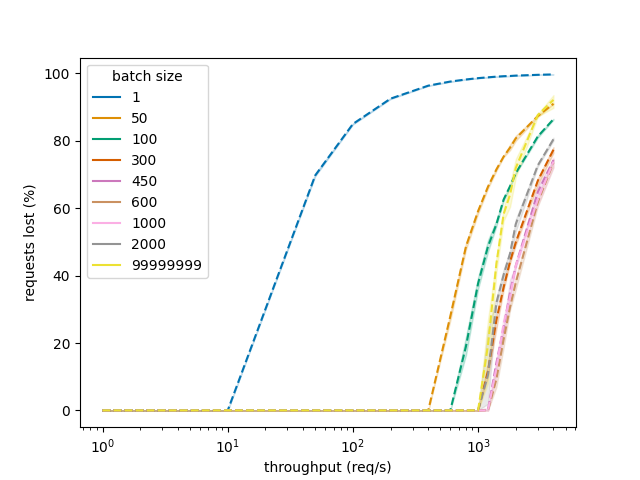
\includegraphics[scale=0.75]{dummy_test/throughputlost.png}
\caption{Benchmarking of Cap'n Proto server \% of failed requests for varying throughputs and message sizes, run for 10s}
\end{figure}

[describe the experiment methodology, present argument, then back up with evidence from figures]
We benchmarked the latency and goodput of sending messages in Cap'n Proto. We varied the size of messages sent in different tests to replicate the behaviour of the algorithm when sending `batches' of many commands, so a message size of 600 means that the message size is approximately that of a message containing 600 commands.

The figures demonstrate that the framework has a severe drop in performance when sending large messages. For a message size of 600 the goodput goes to zero as the throughput increases, meaning that no messages are being responded to.

[``Fundamentally, there are limitations in the RPC framework that give an upper bound on the performance we can hope to achieve, these limitations are evident in our benchmarking of the Cap'n Proto framework\dots'']

\subsection{Tezos Cryptography} \label{tezosbenchmark}
I profiled the important functions of the library with Jane Street's Core\_bench module [citation needed***]. Core\_bench is a micro-benchmarking library used to estimate the cost of operations in OCaml, it runs the operation many times and uses linear regression to try to reduce the effect of high variance between runs.

\begin{table}[!h]
	\centering
	\begin{tabular}{|l|r|}
	\hline
	Function                 & Time (µs) \\ \hline
	Sign                     & 427.87   \\
	Check                    & 1,171.77 \\
	Aggregate (4 sigs)       & 302.90   \\
	Aggregate check (4 sigs) & 1,179.25 \\
	Aggregate (8 sigs)       & 605.38   \\
	Aggregate check (8 sigs) & 1,180.61 \\ \hline
	\end{tabular}
	\caption{Benchmarking of key functions of the Tezos Cryptography library}
\end{table}
% ┌─────────────┬────────────┬─────────┬──────────┬──────────┬────────────┐
% │ Name        │   Time/Run │ mWd/Run │ mjWd/Run │ Prom/Run │ Percentage │
% ├─────────────┼────────────┼─────────┼──────────┼──────────┼────────────┤
% │ sign        │   427.87us │ 144.00w │          │          │     36.24  │
% │ check       │ 1_171.77us │  75.00w │          │          │     99.25  │
% │ agg_4       │   302.90us │ 484.00w │    0.15w │    0.15w │     25.66  │
% │ agg_check_4 │ 1_179.25us │  75.00w │          │          │     99.88  │
% │ agg_8       │   605.38us │ 944.00w │    0.35w │    0.35w │     51.28  │
% │ agg_check_8 │ 1_180.61us │  75.00w │          │          │    100.00  │
% └─────────────┴────────────┴─────────┴──────────┴──────────┴────────────┘

\section{HotStuff implementation benchmarks} \label{hotstuffbenchmarks}

\begin{figure}[h!]
\centering
\includegraphics[scale=0.75]{batch_size_test/throughputgoodput.png}
\caption{Heatmap showing relatively stable latency throughout the course of the experiment. [add parameters!!]}
\label{stableheatmap}
\end{figure}

\begin{figure}[h!]
\centering
\includegraphics[scale=0.75]{batch_size_test/throughputflatency.png}
\caption{Heatmap showing linear growth in latency as the experiment progresses. [add parameters]}
\label{linearheatmap}
\end{figure}

We now analyse the performance and behaviour of the system with different parameters, and under different conditions. We argue that the optimisations described in section \ref{performance} were effective in improving system performance, but there are fundamental limitations caused by the latency costs of Cap'n Proto serialisation (section \ref{capnpbenchmark}) and cryptography (section \ref{tezosbenchmark}).

In most cases, the system exhibits stable latency while goodput is equal to throughput (meaning the system is not overloaded); this is visible in figure [heatmap]. When the throughput exceeds the amount the system can keep up with, there is linear growth in latency as commands queue on the nodes (figure [heatmap]). Since HotStuff is a partially synchronous protocol (section \ref{hotstufftheory}), an increase in latency means that view times increase, decreasing goodput. Once the system is overloaded, the goodput levels off at around its maximum value as throughput is increased.

In our comparison of batch sizes (section \ref{batchsizeseval}) there is evidence that the implementation of batching (section \ref{batching}) was effective, as the system is able to achieve much greater goodput with batch sizes greater than 1 (equivalent to no batching). This section also provides evidence that serialisation latency is a bottleneck, as view times begin to increase exponentially as batch sizes increase, due to messages being larger and taking longer to serialise.

Our study of node counts (section \ref{nodecountseval}) gives further evidence that message serialisation is a bottleneck; higher node counts mean more internal messages being sent, causing a decline in performance due to serialisation costs. This also supports the conclusion that cryptography is a bottleneck, as more nodes means more messages must be signed and aggregated.

In our ablation study (section \ref{ablation}) we compare the performance of the system with different optimisations enabled, demonstrating their effectiveness in increasing goodput, and lowering latency. We also demonstrate that cryptography is a bottleneck by demonstrating the superior performance of the system with cryptography disabled.

In our wide area network (WAN) simulation study (section \ref{minineteval}), we compare the performance of our system running locally, to a simulated mininet network (section \ref{testing}) with link latency similar to what one might find in a wide area network. [we found...]

In our view-change study (section \ref{viewchange}) we demonstrate that the view-change protocol (section \ref{viewchange}) is effective in ensuring the system progresses once a node has died, albeit with a significant performance penalty.

\subsection{Batch sizes} \label{batchsizeseval}

\begin{figure}[h!]
\centering
\includegraphics[scale=0.75]{batch_size_test/throughputgoodput.png}
\caption{Benchmarking of goodput for varying throughputs and batch sizes.}
\label{throughputgoodputbatch}
\end{figure}

\begin{figure}[h!]
\centering
\includegraphics[scale=0.75]{batch_size_test/throughputflatency.png}
\caption{Benchmarking of mean latency while varying throughputs and batch sizes. Discarded result if goodput was not within 5\% of target throughput.}
\label{throughputlatencybatch}
\end{figure}

\begin{figure}[h!]
\centering
\includegraphics[scale=0.75]{batch_size_test/throughputflatency.png}
\caption{Heatmap showing exponential growth in latency as the experiment progresses. [add parameters]}
\label{expheatmap}
\end{figure}

This study compares the performance of the system for varying limits on batch sizes (section \ref{batchsizes}). All experiments were run on a network of 4 nodes.

At lower throughputs where the system is not overloaded, throughput grows linearly with goodput, as the system is able to responds to all incoming requests (figure \ref{throughputgoodputbatch}), with relatively stable latency (figure \ref{stableheatmap}). During this period batches are not filled, so larger throughputs result in larger messages and a slow linear increase in latency due to increasing serialisation latency (figure \ref{throughputlatencybatch}). The system is able to reach a higher goodput before being overloaded if it has a larger batch size, as each view results in more commands being committed; this supports our conclusion that batching is an effective optimisation.

Once throughput is increased enough, batches begin to be filled up and the system is overloaded. This results in the goodput flattening out (figure \ref{throughputgoodputbatch}), as the system cannot handle the volume of requests; commands begin to queue on the nodes and latency increases linearly (figure \ref{linearheatmap}). For higher batch size limits (especially unlimited), goodput declines once the system is overloaded rather than flattening off. This is because the benefits of larger batches are offset by messages becoming larger, causing increased serialisation latency, increased view times, resulting in lower goodput. For large batch sizes, view times increase exponentially, as shown by the growing vertical gaps between commands being committed in figure \ref{expheatmap}.

There is a clear trade-off between larger batch sizes that result in more commands being committed, and batches becoming too large and incurring exponential serialisation latency. The optimum for our system appears to be a batch size of around 600 commands, with a maximum goodput of around 900req/s. (figure \ref{throughputgoodputbatch}).

% There is a trade-off between having larger batches to process more commands, and messages becoming too large and increasing serialisation latency, which is apparent from figure \ref{throughputgoodputbatch}. With small batch sizes each view only commits a small number of commands, leading to low goodputs; an extreme example of this is a batch size of 1 (equivalent to no batching). As batch sizes increase the goodput reached also increases, with goodput peaking at around 700req/s with a batch size of 300 commands. At this point increasing batch size further causes goodput to decrease due to the increased latency of serialising large messages; each view takes longer so less nodes are committed per second (even though each node contains more commands). When the batch size is unlimited messages grow very large as throughput increases, and increased serialisation latency causes goodput to decline.

% Figure \ref{throughputlatencybatch} shows that latency scales linearly with throughput while the system is not overloaded, that is, when the goodput is within 5\% of the target throughput. This is because larger throughputs result in larger message sizes, and increased latency due to serialisation time. 

\subsection{Node counts} \label{nodecountseval}

\begin{figure}[h!]
\centering
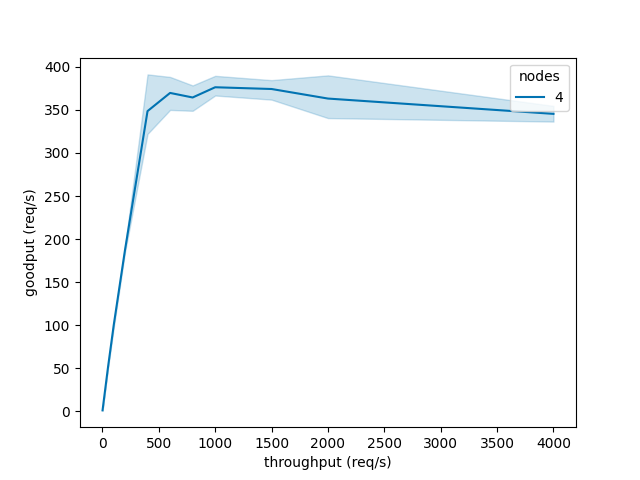
\includegraphics[scale=0.75]{node_count_test/throughputgoodput_nodes.png}
\caption{Benchmarking of goodput for varying throughputs and node counts.}
\label{throughputgoodputnodes}
\end{figure}

\begin{figure}[h!]
\centering
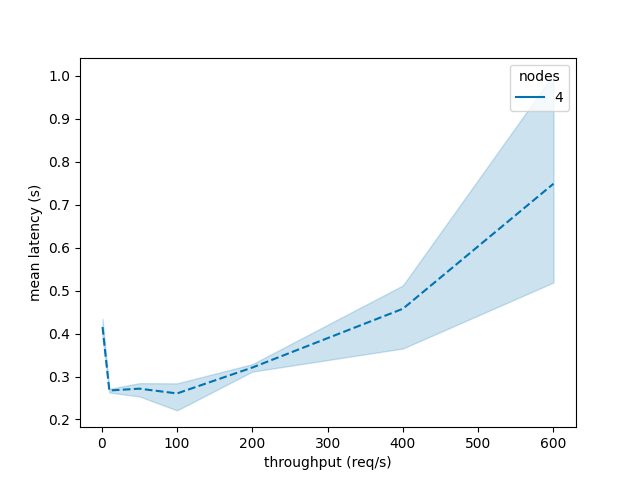
\includegraphics[scale=0.75]{node_count_test/throughputflatency_nodes.png}
\caption{Benchmarking of mean latency while varying throughputs and node counts. Discarded result if goodput was not within 5\% of target throughput.}
\label{throughputlatencynodes}
\end{figure}

This study compares the performance of the system for varying node counts. Node counts were chosen such that $n = 3f + 1$ for some $f$, as choosing another value would decrease performance without any benefit of increased fault-tolerance\footnote{A node count of 2 was also tested as it is the smallest node count where internal messages are exchanged.}. All experiments were run with a batch size of 300.

Figure \ref{throughputlatencynodes} shows that as node count increases, latency increases. This is because larger node counts mean that each view requires more internal messages to be sent to progress. Sending internal messages is expensive due to the latency of serialisation and cryptography, so this results in increased overall latency. Additionally, increasing the node count increases the number of messages that must be signed, and makes aggregating signatures slower (section \ref{tezosbenchmark}). As in our study of batch sizes (section \ref{batchsizeseval}), latency also increases linearly with throughput while the system is not overloaded. Notably the latency for a system of 1 node increases slowly, as there are no internal messages, just client requests and responses.

Figure \ref{throughputgoodputnodes} shows that the larger the node count, the lower the maximum goodput. This is again due to larger node counts resulting in more internal messages, causing more latency since this is a bottleneck. Increased latency causes each view to take longer, reducing the number of requests that can be committed and responded to each second.

\subsection{Ablation study} \label{ablation}

\begin{table}[h]
\centering
\begin{tabular}{|c|c|c|c|c|}
\hline
Version & Chained & Truncation & Filtering & Crypto \\ \hline
1 & \xmark & \xmark & \xmark & \cmark \\ \hline
2 & \cmark & \xmark & \xmark & \cmark \\ \hline
3 & \cmark & \xmark & \cmark & \cmark \\ \hline
4 & \cmark & \cmark & \xmark & \cmark \\ \hline
5 & \cmark & \cmark & \cmark & \cmark \\ \hline
6 & \cmark & \cmark & \cmark & \xmark \\ \hline
\end{tabular}
\caption{Features enabled in different versions.}
\label{versiontable}
\end{table}

\begin{figure}[h!]
\centering
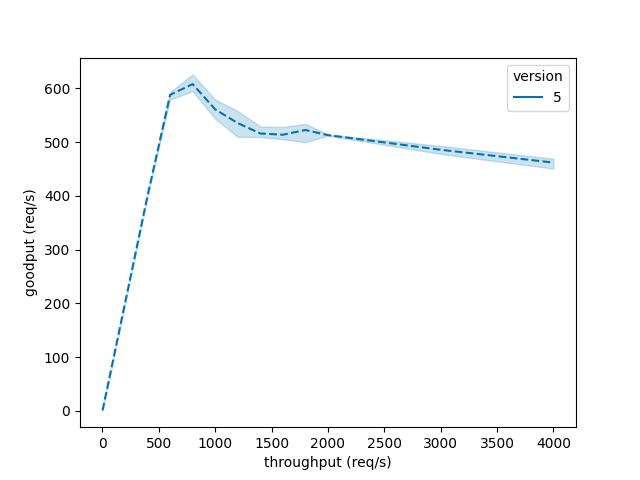
\includegraphics[scale=0.75]{ablation/throughputgoodput_ablation.png}
\caption{Benchmarking of goodput for varying throughputs and implementation versions, run for 10s with 4 nodes unlimited batch size.}
\end{figure}

\begin{figure}[h!]
\centering
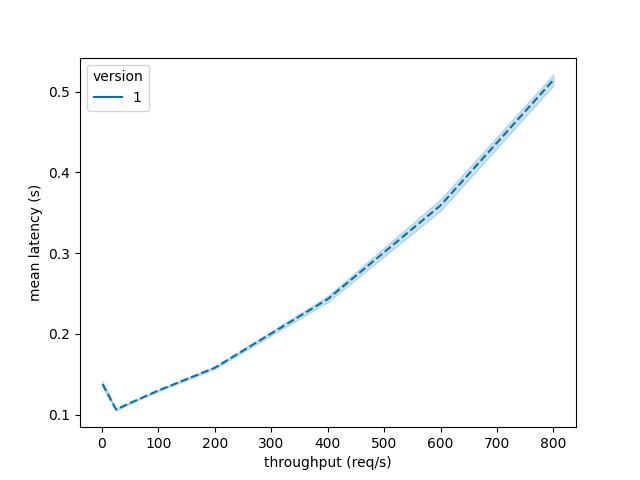
\includegraphics[scale=0.75]{ablation/throughputflatency_ablation.png}
\caption{Benchmarking of mean latency while varying throughputs and implementation versions, run for 10s with 4 nodes unlimited batch size. Discarded result if goodput was not within 5\% of target throughput.}
\end{figure}

This study compares the performance of different versions of the system with different optimisations enabled. The optimisations explored are chaining (section \ref{chaining}), node truncation (section \ref{truncation}), and command filtering (section \ref{sendtoall}). We also compare performance with cryptography disabled. The mapping from version numbers to which features are enabled is given in table \ref{versiontable}. All experiments were run with a network of 4 nodes, and unlimited batch sizes.

\subsection{Wide area network simulation} \label{minineteval}

\begin{figure}[h!]
\centering
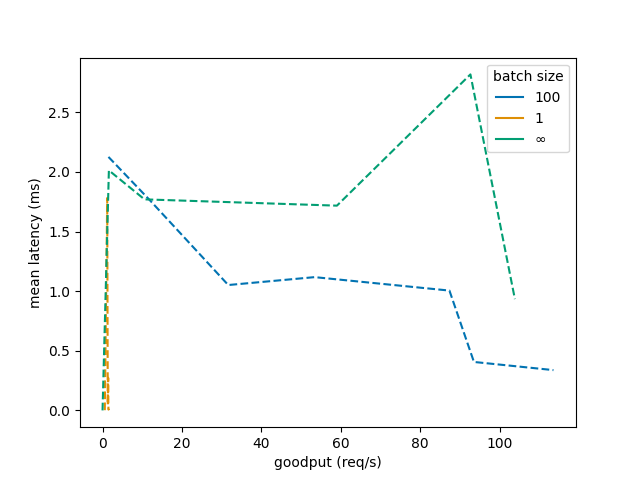
\includegraphics[scale=0.75]{mininet/throughputlatency.png}
\caption{Benchmarking of mean latency while varying throughputs and batch sizes, run for 10s with 100ms network delay.}
\end{figure}

\begin{figure}[h!]
\centering
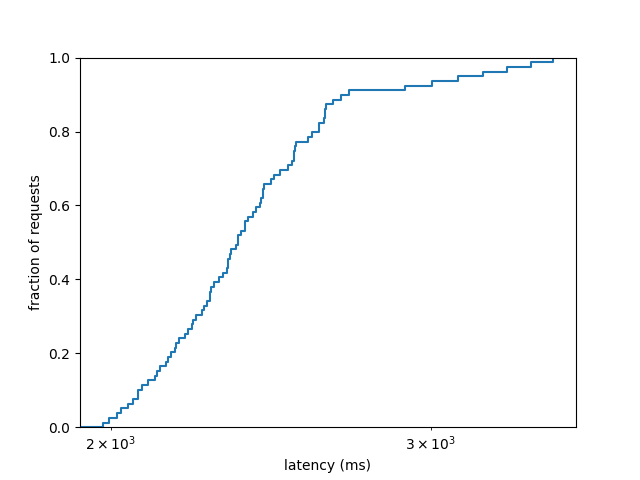
\includegraphics[scale=0.75]{mininet/10tpub_cumlatency.png}
\caption{Cumulative latency plot for experiment with a throughput of 10req/s and unlimited batch size, run for 10s with 100ms network delay.}
\end{figure}

[Give ablation graphs comparing the performance with 100ms delay, and without.]

\subsection{View-changes} \label{viewchangeeval}

\begin{figure}[h!]
\centering
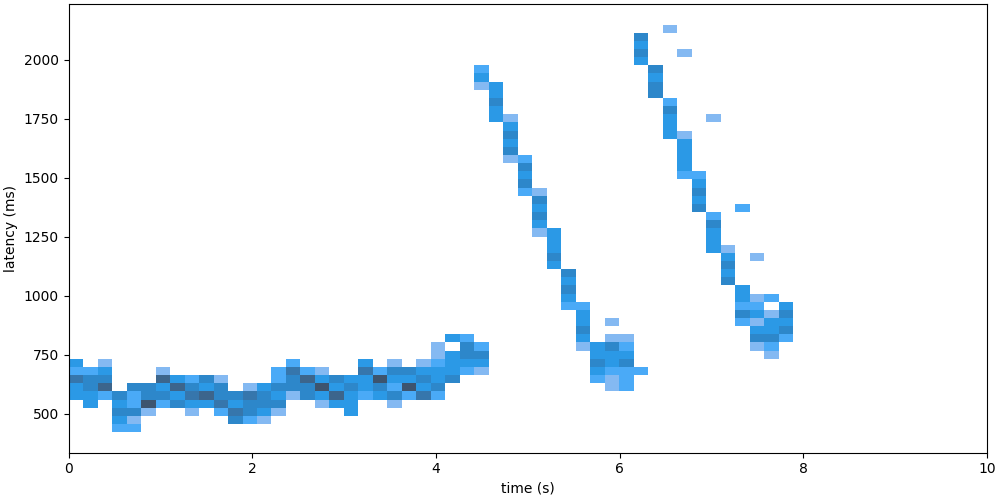
\includegraphics[scale=0.5]{viewchange/test7_100_7_100_timelatencyheatmap.png}
\caption{Heatmap showing distribution of latencies with a node being killed 5s in. Run for 10s with 7 nodes and a batch size of 100.}
\end{figure}
% Clone github.com/cjen1/reckon

% ```
% # This is likely to take a while
% make reckon-mininet

% docker run -it --privileged -e DISPLAY --network host --name reckon-mininet cjen1/reckon:latest bash

% # Set up mininet net with a single switch and 3 nodes
% # drops you into a cli (you can also use python scripting)
% mn --topo single,3

% # observe no delay between nodes
% mininet> h1 ping h2
% mininet> <Ctrl-C>/<Ctrl-D> to exit

% # syntax is `mininet> <node> <command>`
% # I run screens on each node and then attach to those from outside mininet to run the tests in different terminal screens. (Tmux doesn't work correctly afaicr)

% mininet> h1 screen -dmS node_h1 bash

% #Then in another terminal session
% docker exec -it reckon-mininet bash
% screen -r node_h1
% <whatever commands you want to run on that emulated node>

% #Similarly for the other nodes
% ```